\documentclass[conference]{IEEEtran}
\IEEEoverridecommandlockouts

\usepackage{cite}
\usepackage{amsmath,amssymb}
\usepackage{graphicx}
\usepackage{textcomp}
\usepackage{xcolor}
\usepackage{listings}
\usepackage{booktabs}
\usepackage{url}
\usepackage[hidelinks]{hyperref}

\graphicspath{{../dissertation/images/}}

\lstdefinelanguage{Kotlin}{
  keywords={val, var, fun, to, true, false},
  sensitive=true,
  comment=[l]{//},
  string=[b]"
}
\lstdefinelanguage{json}{
  string=[b]"
}
\lstset{
  basicstyle=\ttfamily\scriptsize,
  keywordstyle=\bfseries,
  stringstyle=\color{black!70},
  columns=fullflexible,
  keepspaces=true,
  frame=tb,
  breaklines=false,
  captionpos=b,
  aboveskip=6pt,
  belowskip=4pt
}

\hyphenation{Quick-FaaS Omni-Flow}

\begin{document}

\title{Unified Orchestration of Serverless Workflows\\with QuickFaaS and OmniFlow}

\author{\IEEEauthorblockN{Pedro Carvalho}
\IEEEauthorblockA{\textit{ISEL -- Instituto Superior de Engenharia de Lisboa}\\
\textit{Instituto Polit\'ecnico de Lisboa}\\
Lisbon, Portugal}
\and
\IEEEauthorblockN{Jos\'e Sim\~ao}
\IEEEauthorblockA{\textit{ISEL -- Instituto Superior de Engenharia de Lisboa}\\
\textit{Instituto Polit\'ecnico de Lisboa}\\
Lisbon, Portugal}
\and
\IEEEauthorblockN{Filipe Freitas}
\IEEEauthorblockA{\textit{ISEL -- Instituto Superior de Engenharia de Lisboa}\\
\textit{Instituto Polit\'ecnico de Lisboa}\\
Lisbon, Portugal}
}

\maketitle

\begin{abstract}
Serverless applications are commonly built from functions deployed on a Function-as-a-Service
(FaaS) platform and composed by a managed workflow engine. Portable tooling exists for each half:
QuickFaaS deploys cloud-agnostic functions, and OmniFlow compiles a Kotlin workflow DSL into AWS
Step Functions or Google Cloud Workflows definitions. Used together, however, they leave the
developer to deploy every function first and copy its provider-assigned endpoint into the workflow
by hand. This paper unifies the two tools so that a single workflow definition drives both
deployments. A call step names a function it owns through an \texttt{internalFunction} construct;
at deployment time a three-level resolution ladder binds that logical name to a concrete endpoint,
using a per-provider Function Registry validated against the live function, provider discovery
across regions, and, only when the function is confirmed to be absent, deployment through
QuickFaaS. To make the unification available on both providers OmniFlow targets, QuickFaaS is
extended with an AWS Lambda provider and its GCP provider is moved to Cloud Run functions. Unit
tests on both providers show that the ladder takes the expected decision in all 18 situations it
can meet, including stale entries, ambiguous names and inaccessible regions. Microbenchmarks show
that resolving a 200-call workflow costs $29\,\mu$s on AWS and $199\,\mu$s on GCP of local work,
growing linearly with the number of internal calls, and that a current registry keeps provider
traffic at one request per call. For one function on GCP, the integrated procedure takes four
developer steps instead of nine, and no value has to be copied by hand.
\end{abstract}

\begin{IEEEkeywords}
serverless computing, function-as-a-service, workflow orchestration, deployment automation,
vendor lock-in, AWS Lambda, Google Cloud
\end{IEEEkeywords}

% =====================================================================
\section{Introduction}
\label{sec:intro}

Serverless computing lets developers deploy fine-grained, stateless functions that run on demand,
scale automatically and are billed per execution~\cite{serverlessComputing,jonas2019cloudProgramming}.
Because a function holds no state and cannot directly call another, non-trivial applications lift
their control flow into a workflow engine, such as AWS Step Functions or Google Cloud
Workflows~\cite{aws_stepfunctions_concepts,gcp_workflows_overview}. Both layers expose the
application to vendor lock-in: function code is coupled to each provider's signatures and
packaging, and workflow logic to each provider's orchestration language.

Two tools developed at ISEL address these layers separately. \emph{QuickFaaS} deploys functions
written against a uniform, provider-agnostic programming model~\cite{rodrigues2022quickfaas}.
\emph{OmniFlow} defines workflows in a Kotlin DSL and compiles them into provider-native
definitions~\cite{costa2023omniflow,silva2025advanced}. Each automates one half of the deployment
of a serverless application, but the two halves remain disconnected. An OmniFlow call step needs a
concrete \texttt{host} and \texttt{path}, and that endpoint exists only after the function has
been deployed: on AWS it is an ARN containing the region and account, and on GCP a URL assigned by
the provider. The developer must therefore deploy every function first, read its endpoint and
paste it into the workflow. Nothing checks the pasted value before the workflow runs, and the
procedure is repeated for every function, region, account and provider the workflow is deployed
to. Moreover, QuickFaaS supported only GCP and Azure, so the two tools overlapped on a single
provider.

This work closes that gap. Two research questions guide it:
\begin{itemize}
  \item \textbf{RQ1 (feasibility and correctness):} can OmniFlow, from a single workflow
  definition, bind each internal function call to the right endpoint at deployment time, on both
  AWS and GCP, and deploy a function through QuickFaaS only when it is confirmed to be missing?
  \item \textbf{RQ2 (overhead):} how much local work does this resolution add to a deployment,
  how does it grow with the number of calls and the registry size, and how many requests does it
  send to the provider?
\end{itemize}

The contributions are: (i)~a call model that separates \emph{internal} functions, owned by the
developer and named logically, from \emph{external} ones called through a literal endpoint;
(ii)~a per-provider Function Registry and a three-level, fail-fast resolution ladder that binds
logical names to endpoints at deployment time; (iii)~an AWS Lambda provider for QuickFaaS, with a
matching deployer in OmniFlow, and a GCP provider moved to Cloud Run functions; (iv)~a prototype
and a case study in card-payment fraud detection deployed to both providers; and (v)~an evaluation
of the ladder's decisions and of its cost. A preliminary version of the architecture was
presented in~\cite{carvalho2026towards}; this paper reports the complete design, the resolution
ladder, the AWS support and the evaluation.

Section~\ref{sec:background} introduces the two base tools and Section~\ref{sec:related} the
related work. Section~\ref{sec:solution} presents the proposed solution and
Section~\ref{sec:impl} its implementation. Section~\ref{sec:case} summarises the case study,
Section~\ref{sec:eval} the evaluation, and Section~\ref{sec:concl} concludes.

% =====================================================================
\section{Background}
\label{sec:background}

\subsection{QuickFaaS}
QuickFaaS is a Kotlin desktop tool whose goal is to write a function once and deploy it to several
FaaS platforms without changing its code~\cite{rodrigues2022quickfaas}. Developers implement a
\emph{hook} function against generic request and response types (\texttt{HttpRequestQf},
\texttt{HttpResponseQf}); for each provider and trigger, QuickFaaS supplies a \emph{template}
function that serves as the platform entry point, adapts the provider's event to the generic types
and calls the hook. Deployment follows a ZIP strategy: the hook, the template and the QuickFaaS
libraries are built and packaged into an archive, uploaded to a storage bucket and deployed from
there. A JSON descriptor names the provider, project, function name, region, bucket, runtime,
trigger and source file. Once the function is deployed, the developer still has to grant invoke
permission, read the generated endpoint and use it wherever the function is called.

\subsection{OmniFlow}
OmniFlow is a client-side Kotlin library for defining serverless workflows independently of any
provider schema~\cite{costa2023omniflow,silva2025advanced}. A type-safe builder DSL produces a
provider-agnostic tree of steps (execution steps such as \texttt{call} and \texttt{assign},
conditional, iteration and parallel steps), which provider-specific renderers traverse depth-first
to emit an Amazon States Language (ASL) state machine or a Cloud Workflows YAML definition; a
provider deployer then submits it. A \texttt{call} step is an HTTP request with a method, a
\texttt{host}, a \texttt{path}, optional query parameters and body, and a result variable. Its
endpoint therefore has to be known when the workflow is written, and this is the manual
synchronisation that this work removes.

% =====================================================================
\section{Related Work}
\label{sec:related}

\emph{Infrastructure-as-Code (IaC) tools} automate deployment. CloudFormation and the AWS
CDK~\cite{awsCloudFormation,awsCdk} are tied to AWS; Terraform, Pulumi and the Serverless
Framework~\cite{terraform,pulumi,serverlessFramework} are provider-agnostic as tools, but functions
are still described through provider-specific resources. These tools already bind a workflow to a
function at deployment time: AWS SAM substitutes \texttt{!GetAtt MyFunction.Arn} into a state
machine definition~\cite{awsSamStateMachine}, Terraform interpolates
\texttt{aws\_lambda\_function.x.arn}~\cite{terraformSfnStateMachine} and Pulumi passes outputs as
inputs~\cite{pulumiInputsOutputs}, each creating the function before the workflow. They bind only
functions declared (or explicitly looked up in a given region~\cite{terraformLambdaDataSource,pulumiLambdaGetFunction})
in the same configuration, and the workflow remains written in one provider's language.
CODE~\cite{ristov2024code} deploys a function once across the regions of several providers but
leaves the deployment of workflows as future work.

\emph{Portable runtimes} such as OpenFaaS~\cite{openFaaS} run functions on their own container
platform rather than on provider-native FaaS. SEAPORT~\cite{yussupov2020seaport} \emph{measures}
the portability of serverless applications rather than providing it.

\emph{Workflow frameworks} such as FaaSFlow~\cite{li2022faasflow} and
Triggerflow~\cite{garciaLopez2020triggerflow} target execution efficiency and event-driven
orchestration. Serverless Workflow~\cite{serverlessWorkflowSpec}, Temporal~\cite{temporalPlatform},
FaaSr~\cite{park2024faasr} and Serverless Multicloud~\cite{zhao2022supporting} provide portable
workflow definitions or APIs, but execute them on their own runtime or middleware. The closest in
intent is AFCL/xAFCL~\cite{ristov2021afcl,ristov2023xafcl}: a provider-independent workflow
language whose functions may run on several FaaS systems. Each function in an AFCL workflow,
however, carries the concrete ARN or URL it invokes, every function must be deployed beforehand,
and the workflow is run by the xAFCL engine rather than by a provider-native service.

\emph{Service registries} such as AWS Cloud Map and Consul~\cite{awsCloudMap,consulServiceDiscovery}
map logical names to endpoints, but they are consulted at run time by the caller and deploy nothing.

Table~\ref{tab:related} summarises the comparison. No surveyed work combines deployment-time
binding with a workflow definition that deploys to more than one provider-native engine, functions
written against a provider-agnostic model, and on-demand deployment of missing functions.

\begin{table}[t]
  \centering
  \caption{Positioning (Y = yes, P = partial, -- = no). D: deployment automation; FP/WP: function
  and workflow portability; B: deployment-time binding; S: discovery by name; N: provider-native
  execution.}
  \label{tab:related}
  \footnotesize
  \setlength{\tabcolsep}{3.2pt}
  \begin{tabular}{|l|c|c|c|c|c|c|}
    \hline
    \textbf{Approach} & \textbf{D} & \textbf{FP} & \textbf{WP} & \textbf{B} & \textbf{S} & \textbf{N} \\
    \hline
    CloudFormation/SAM, CDK      & Y & -- & -- & Y & -- & Y \\
    \hline
    Terraform, Pulumi            & Y & P  & -- & Y & P  & Y \\
    \hline
    Serverless Framework         & Y & P  & -- & Y & -- & Y \\
    \hline
    CODE~\cite{ristov2024code}   & Y & Y  & -- & -- & -- & Y \\
    \hline
    OpenFaaS                     & Y & Y  & -- & -- & -- & -- \\
    \hline
    SEAPORT                      & -- & -- & -- & -- & -- & -- \\
    \hline
    FaaSFlow, Triggerflow        & -- & -- & P/Y & -- & -- & -- \\
    \hline
    AFCL/xAFCL                   & -- & -- & Y & -- & -- & -- \\
    \hline
    Serverless Workflow, Temporal & -- & -- & Y & -- & -- & -- \\
    \hline
    FaaSr                        & P & P  & Y & -- & -- & -- \\
    \hline
    Cloud Map, Consul            & -- & -- & -- & -- & Y & -- \\
    \hline
    \textbf{This work}           & Y & Y  & P\textsuperscript{a} & Y & P\textsuperscript{b} & Y \\
    \hline
  \end{tabular}\\[2pt]
  \parbox{\columnwidth}{\scriptsize \textsuperscript{a}Two providers (AWS, GCP).
  \textsuperscript{b}Across the regions of one account or project; no shared registry.}
\end{table}

% =====================================================================
\section{Proposed Solution}
\label{sec:solution}

\subsection{Architecture}
Figure~\ref{fig:arch} shows the integrated toolchain. A single workflow definition drives both
concerns: each OmniFlow provider deployer delegates the resolution of internal calls to a
provider-specific resolver, backed by a registry file of its own. When a function has to be
deployed, the resolver invokes QuickFaaS, which gains an AWS provider. The end-to-end flow is:
(1)~the developer writes the workflow and one QuickFaaS descriptor per internal function;
(2)~OmniFlow walks the workflow tree and, for each internal call, (3)~resolves the endpoint from
the registry, discovers it on the provider or deploys it through QuickFaaS; (4)~metadata obtained
by discovery or deployment, or refreshed after drift, is written to the registry; and (5)~the
resolved workflow is rendered and deployed. External calls bypass the registry.

\begin{figure*}[t]
  \centering
  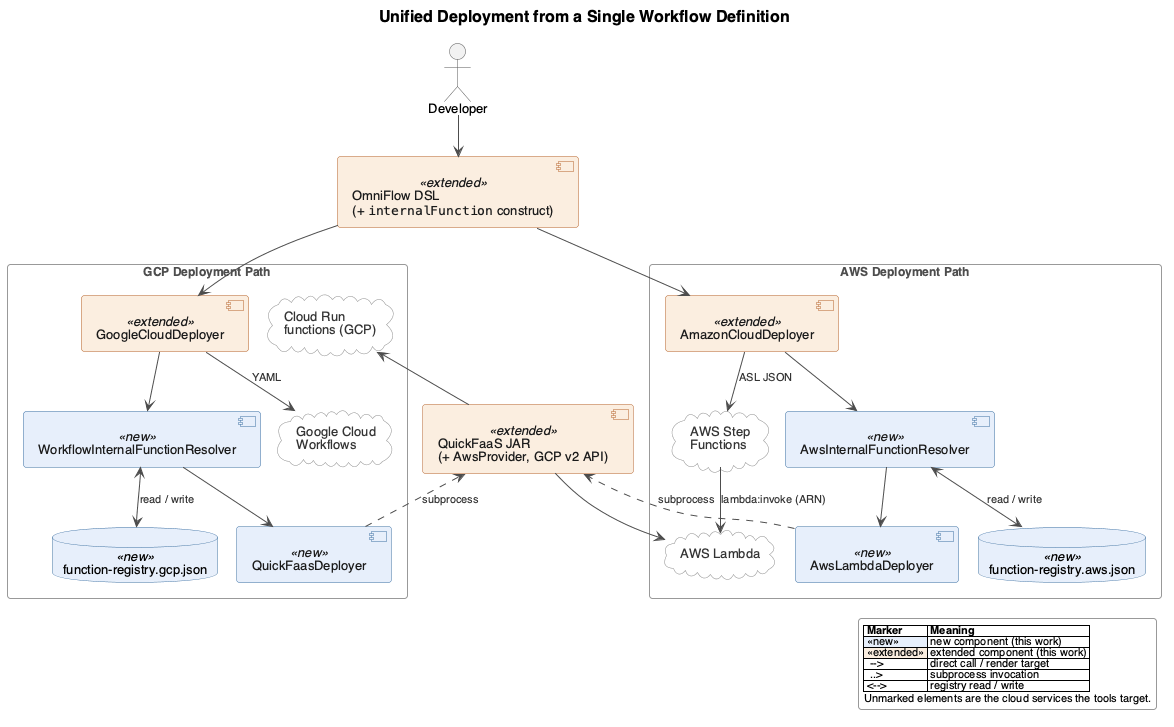
\includegraphics[width=0.82\textwidth]{architecture/architecture-after.png}
  \caption{Unified deployment from a single workflow definition. Components marked
  \emph{new}/\emph{extended} are the contribution of this work.}
  \label{fig:arch}
\end{figure*}

\subsection{Call Model}
The OmniFlow \texttt{call} step gains an alternative to \texttt{host}/\texttt{path}: the
\texttt{internalFunction(name, deploymentDescriptorPath)} construct. Which form a call uses depends
on who owns the target. A function whose code the developer owns, and may deploy, is
\emph{internal}; it is named by a stable logical identifier, the \texttt{functionRef}, and may
point to the QuickFaaS descriptor that builds it. A function or API the developer does not own is
\emph{external}: it keeps a literal endpoint, is never deployed and is not recorded in the
registry. The two forms are mutually exclusive, checked when the DSL is built and again at
resolution time. Listing~\ref{lst:wf} shows a workflow with one call of each kind; the internal call
names no host, region or provider.

\begin{lstlisting}[language=Kotlin,caption={A workflow with an internal and an external call.},label={lst:wf}]
val wf = workflow {
  name("FraudPipeline")
  params("args")
  steps(
    step { name("fraud-check")
      context(call {
        method(GET)
        internalFunction("fraud-check",
                         "./deploy/fraud-check.json")
        result("fraudResult") }) },
    step { name("external-risk-api")
      context(call {
        method(POST)
        host("api.partner.example")
        path("/v1/risk-score")
        result("riskResult") }) })
  result("riskResult")
}
\end{lstlisting}

\subsection{Function Registry}
The registry is a JSON file per provider (\texttt{function-registry.gcp.json},
\texttt{function-registry.aws.json}) that maps each \texttt{functionRef} to the metadata needed to
invoke it: \texttt{serviceName}, the function's name on the provider, and \texttt{url}, an opaque,
provider-interpreted endpoint (Listing~\ref{lst:registry}). On GCP, \texttt{url} is the function's
HTTPS address and \texttt{serviceName} the full resource name of the Cloud Run service behind it;
on AWS, \texttt{url} is the Lambda ARN. The key is the bare \texttt{functionRef} while it is
unambiguous, and is qualified as \texttt{"region/functionRef"} when the same name exists in more
than one region. No credentials or deployment parameters are stored, and the file is written only
by the integration. Keeping the endpoint in a single opaque field meant that adding AWS did not
change the schema: only the resolver and renderer that interpret the field are provider-aware.

\begin{lstlisting}[language=json,caption={Registry entries on each provider (abridged).},label={lst:registry}]
function-registry.aws.json:
{ "updatedAt": "2026-09-28T14:18:54Z",
  "functions": { "eu-west-1/fraud-check": {
    "serviceName": "fraud-check",
    "url": "arn:aws:lambda:eu-west-1:111111111111:
            function:fraud-check" } } }
function-registry.gcp.json:
{ "updatedAt": "2026-09-28T09:50:43Z",
  "functions": { "europe-west1/fraud-check": {
    "serviceName": "projects/p/locations/
                    europe-west1/services/fraud-check",
    "url": "https://fraud-check-a1b2c3-ew.a.run.app" } } }
\end{lstlisting}

\subsection{Resolution Ladder}
Each internal call goes through a three-level ladder that stops at the first level that succeeds,
so that the cheapest action is preferred and deployment is a last resort:
\begin{enumerate}
  \item \textbf{Level 1 (registry).} The \texttt{functionRef} is looked up (exact match, then a
  suffix match on \texttt{"region/functionRef"}). A hit is validated against the live function in
  the place the entry records (the region inside the ARN, or the Cloud Run resource name). A
  changed endpoint refreshes the entry; a function deleted from its region is searched for in the
  other regions and, if not found, its entry is removed and the deployment aborts.
  \item \textbf{Level 2 (discovery).} On a miss, the provider is queried across the candidate
  regions (Cloud Run services of the project on GCP, every region enabled for the account on AWS),
  starting with the workflow's own region; a \texttt{"region/functionRef"} reference queries one
  region only. A function found in exactly one region is registered and used, without deployment.
  \item \textbf{Level 3 (deployment).} Only when the function is absent from the registry and from
  every region, and the call supplied a descriptor, is QuickFaaS invoked; the returned endpoint is
  registered and used.
\end{enumerate}

The ladder fails fast, and every failure is reported before any artifact is rendered. An
unresolvable function (absent, with no descriptor), an ambiguous name (found in several regions),
a stale entry that cannot be rediscovered, and an absence that cannot be confirmed because some
region was inaccessible all abort the deployment, even when a descriptor is present. QuickFaaS
therefore never deploys a function that may already exist. The ladder never updates an existing
function either: it deploys only missing ones. Re-deploying a workflow is idempotent, since the
second run is a Level 1 hit and consults no descriptor.

\textbf{Static binding.} The resolved endpoint is written into the rendered workflow, and the
deployed workflow never consults the registry. An endpoint that changes afterwards is picked up on
the next workflow deployment, when Level 1 detects the drift. Endpoints change less often than
code: updating a Lambda in place keeps its ARN, and redeploying a Cloud Run function under the same
name and region keeps its URL.

\subsection{Design Rationale}
Only OmniFlow knows which functions a workflow references, so orchestration lives on its side, and
QuickFaaS acts as the deployment mechanism it invokes on demand. The alternative of running both as
long-lived communicating services was rejected: neither is a service, credentials would have to
cross a trust boundary, and a local, sequential, short-lived task gains nothing from a distributed
protocol. Deployment is reached through an \texttt{InternalFunctionDeployer} strategy with one
implementation per provider, each running the unmodified QuickFaaS JAR as a subprocess, which keeps
QuickFaaS a separately built tool (Gradle, Kotlin 1.6) outside OmniFlow's Maven build.

% =====================================================================
\section{Implementation}
\label{sec:impl}

\subsection{Resolvers and Registry Store}
The registry is accessed through \texttt{FunctionRegistryStore}, which reads, looks up, inserts
and removes entries. Two resolvers implement the ladder: \texttt{WorkflowInternalFunctionResolver}
on GCP, over the Cloud Run v2 API, and \texttt{AwsInternalFunctionResolver} on AWS, over the Lambda
API, with regions listed through EC2 \texttt{DescribeRegions}. Both traverse the workflow tree,
including branches, iterations and parallel blocks, and intercept only calls that carry an
\texttt{internalFunction}. The store keeps no cache, so each resolver reads the registry once per
resolution into an in-memory snapshot, resolves every call against it, and keeps the snapshot in
sync with its own writes. If the registry file is missing, a bootstrapper rebuilds it by listing the
functions already deployed on the provider. When validating a hit, a lookup refused by the provider
(an authorization failure) aborts, since it says nothing about whether the function exists.

\subsection{Cloud Run Functions on GCP}
The GCP resolver validates and discovers functions through the Cloud Run API, but the original
QuickFaaS created first-generation Cloud Functions, which are not Cloud Run services. Its GCP
provider was therefore moved to the Cloud Functions v2 API, whose functions are backed by a Cloud
Run service~\cite{gcpFunctionsVersionComparison}. Deployment becomes a long-running operation: the
provider waits for the \texttt{ACTIVE} state, reads the \texttt{run.app} URL from
\texttt{serviceConfig} (it carries a provider-generated hash and cannot be composed), and grants
\texttt{roles/run.invoker} on the backing service. OmniFlow's \texttt{QuickFaasDeployer} then
registers the full resource name and the URL.

\subsection{AWS Lambda Support}
The QuickFaaS \texttt{AwsProvider} implements the existing provider abstractions. It uploads the
ZIP to the S3 bucket named in the descriptor, creates the function (or updates its code), with the
provider-agnostic \texttt{AwsHttpTemplate} as handler, and waits until it is active. A Lambda must
live in the region of its code bucket, so the provider reads that region
(\texttt{GetBucketLocation}) and pins its client to it.

On the OmniFlow side, \texttt{AwsLambdaDeployer} does the work that has no GCP equivalent. It
resolves the execution role, creating a managed role when the descriptor leaves
\texttt{iamRoleArn} as a placeholder, or repairing the trust policy of the one it names. It then
runs QuickFaaS with retries to absorb IAM eventual consistency, waits for the function to become
\texttt{Active}, grants Step Functions permission to invoke it and returns its ARN.

\subsection{Runtime Invocation}
On AWS, an internal call is rendered as a native \texttt{lambda:invoke} task whose
\texttt{FunctionName} is the resolved ARN (Listing~\ref{lst:state}), which avoids request signing
and keeps invocation within the AWS control plane; external calls keep the
\texttt{apigateway:invoke} form. Because the QuickFaaS Lambda template reads only query parameters,
an internal AWS call that declares a body is rejected before the ladder runs. On GCP, the resolved
URL is split into host and path, and the call is rendered as an ordinary \texttt{http} call,
authenticated with an OIDC token for the workflow's service account.

\begin{lstlisting}[language=json,caption={Step Functions state rendered for an internal call.},label={lst:state}]
"fraud-check": {
  "Type": "Task",
  "Resource": "arn:aws:states:::lambda:invoke",
  "Parameters": { "FunctionName": "arn:aws:lambda:
      eu-west-1:111111111111:function:fraud-check" },
  "ResultSelector": { "fraudResult.$": "$.Payload" },
  "ResultPath": "$.fraud-check",
  "Next": "external-risk-api" }
\end{lstlisting}

% =====================================================================
\section{Case Study: Card-Payment Fraud Screening}
\label{sec:case}

A bank authorizes card payments through a \texttt{PaymentAuthorization} workflow. Two internal
functions owned by its fraud team, \texttt{fraud-check} and \texttt{risk-score}, score each
transaction; a \texttt{switch} step declines flagged or high-risk transactions; and an external
call reports the decision to the core banking system. The scenario reflects two requirements:
an exit strategy for information and communication technology (ICT) services supporting critical
functions, as the Digital Operational Resilience Act (DORA) requires of EU
financial entities~\cite{dora2022}; and a record of which endpoint each deployment was bound to.

Two deployments were run on 28 September 2026: one to an AWS account and one to a GCP project. On AWS, with AWS descriptors and the AWS deployer, the registry is bootstrapped from
the account, and both scoring calls miss at Levels 1 and 2 and reach Level 3. QuickFaaS deploys the
two Lambda functions, their ARNs are stored in the \texttt{url} field, and the state machine is
created. To illustrate the exit strategy, the same workflow is also deployed to a second provider:
on GCP, with GCP descriptors and the GCP deployer, a separate registry is bootstrapped and
the same \texttt{functionRef}s resolve to \texttt{run.app} URLs, while the workflow definition
stays unchanged. On each provider, a second deployment, run after deleting the workflow because
OmniFlow's deployers cannot update one, bound both calls at Level 1 and left the registry
byte-identical, and three transactions produced the expected decisions. The runs used
region-qualified references, so the registries are keyed as in Listing~\ref{lst:registry}
(abridged, with placeholder identifiers).

The case study also exposed two defects in OmniFlow's AWS renderer, which this work fixed. An
\texttt{assign} step became a \texttt{Pass} state whose result replaced the whole state document,
so the transaction was no longer available to the final call; a single-variable \texttt{assign} now
writes only that variable, while one of several variables still replaces the state. And the query
parameters of a Lambda call were wrapped in \texttt{States.Array}, so a hook received
\texttt{"[120]"}; they are now plain strings. The scenario remains illustrative rather than
production-ready (Section~\ref{sec:concl}).

% =====================================================================
\section{Evaluation}
\label{sec:eval}

The evaluation exercises only local operations: building and traversing workflows, resolving calls,
reading and writing the registry, and packaging a bundle. Calls to the cloud are excluded because
they are dominated by provider latency (deploying a workflow and its functions takes minutes,
whether or not the tools are integrated) and are non-deterministic. Correctness tests replace the
provider with test doubles, and provider requests are counted from the implementation.

\subsection{Correctness of the Ladder (RQ1)}
Each resolver has a unit-test suite that resolves a small workflow in every situation the ladder
can meet. The provider is replaced by a lookup that answers \emph{found}, \emph{not found} or
\emph{access denied} per region and by a deployer that records its invocations. The registry is not simulated: the
tests use the same registry code as a real deployment, which reads and writes a JSON file in a
directory created empty for each test. Table~\ref{tab:correct} lists the situations. All 46 resolver tests (23 per provider)
and the two bootstrap tests pass: every internal call is bound to the registered, current or
discovered endpoint, and a function is deployed only when it is absent everywhere and every region
could be checked.

\begin{table}[t]
  \centering
  \caption{Situations covered by the resolver tests (both providers unless marked); observed
  behaviour matches the expected one in every case.}
  \label{tab:correct}
  \footnotesize
  \setlength{\tabcolsep}{3pt}
  \begin{tabular}{|p{0.44\columnwidth}|p{0.46\columnwidth}|}
    \hline
    \textbf{Situation} & \textbf{Expected behaviour} \\
    \hline
    Valid registry entry & bound to registered endpoint \\
    \hline
    Entry whose endpoint changed & entry refreshed; bound to current endpoint \\
    \hline
    Entry for a function gone from its region & rediscovered and replaced, or removed and abort \\
    \hline
    Validation denied by provider & abort; entry kept \\
    \hline
    Miss, found in one region & bound and registered \\
    \hline
    Found in several regions & abort (ambiguous) \\
    \hline
    \texttt{region/name} reference & only that region queried \\
    \hline
    All regions inaccessible, not found & abort with distinct error \\
    \hline
    Not found, descriptor given & deployed once; registered; bound \\
    \hline
    Not found, some regions inaccessible & abort; nothing deployed \\
    \hline
    Not found, no descriptor & abort; nothing deployed \\
    \hline
    Calls in branches, loops, parallel & all resolved \\
    \hline
    External calls & left unchanged \\
    \hline
    Both \texttt{internalFunction} and host/path & rejected before the ladder \\
    \hline
    Internal call with a body (AWS) & rejected; nothing deployed \\
    \hline
    Several internal calls & registry read once \\
    \hline
    \texttt{cloudfunctions.net} entry (GCP) & validated via Cloud Run; live URL bound \\
    \hline
    Registry file missing & rebuilt from the provider \\
    \hline
  \end{tabular}
\end{table}

\subsection{Resolution Overhead (RQ2)}
Benchmarks use JMH~1.37 in average-time mode, with three forks, three warm-up and five one-second
measurement iterations, on an idle Apple Silicon laptop. For half the measurements the 99.9\%
confidence interval is under 1\% of the score, and for nine out of ten under 6\%. $N$ denotes the
number of calls, $I$ the internal ones, $F$ the distinct functions and $R$ the registry entries.
The comparison of per-call reads and a single read uses a reference resolver written for the
benchmarks, which resolves calls from the registry without validating them against the provider;
the production resolvers are the classes OmniFlow runs when it deploys a workflow.

\textbf{Per-call reads versus a single read.} A resolver that re-reads the registry on every call
pays, per call, about $10.3\,\mu$s of fixed I/O and parsing plus $0.17\,\mu$s per entry, so the
fixed cost dominates below $R\approx60$. Its total grows with the product $N\cdot R$. Reading the
registry once into a snapshot makes the cost one read plus about $0.23\,\mu$s per internal call:
with $R{=}1000$, resolution stays between $182$ and $184\,\mu$s as $N$ grows from 1 to 200, whereas
per-call reads reach $36.7$\,ms at $N{=}200$, a $200\times$ speedup.

\begin{figure*}[t]
  \centering
  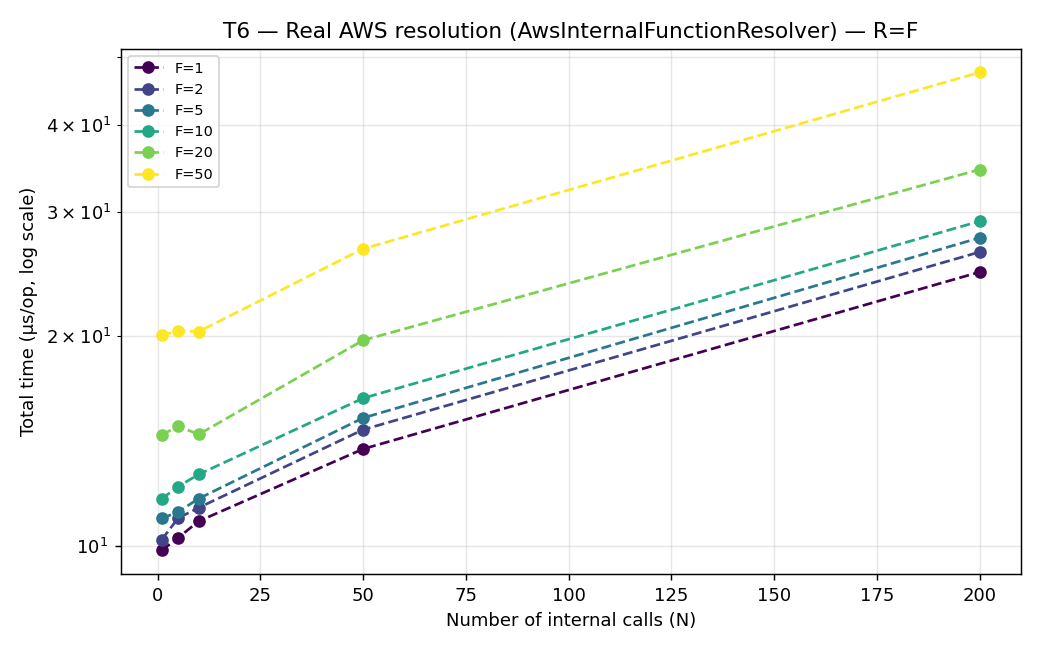
\includegraphics[width=0.49\textwidth]{benchmarks/T6_aws_internal_resolution.png}\hfill
  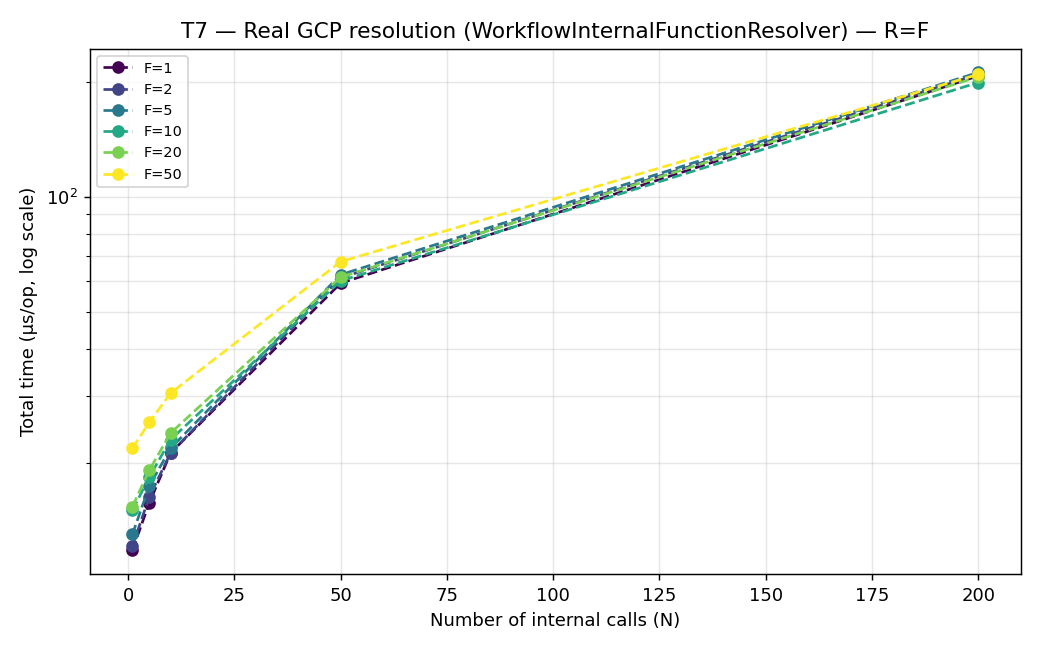
\includegraphics[width=0.49\textwidth]{benchmarks/T7_google_internal_resolution.png}
  \caption{Resolution time of the production resolvers on AWS (left) and GCP (right) against the
  number of internal calls $N$, one curve per number of distinct functions $F$, with $R{=}F$
  (logarithmic vertical axis). Both start from one registry read and grow linearly with $N$; the
  GCP curves rise more steeply because every call goes through the Cloud Run client.}
  \label{fig:t67}
\end{figure*}

\textbf{Production resolvers.} Both production resolvers use the snapshot and show the same shape
(Fig.~\ref{fig:t67}, Table~\ref{tab:t67}). With $R{=}F$, the per-call work is $0.07$--$0.14\,\mu$s on AWS and about
$0.95\,\mu$s on GCP, where every hit goes through the real Cloud Run client (building the request,
obtaining a token and parsing a locally answered response; only the network round trip is
excluded). A 200-call workflow against ten functions costs $29.1\,\mu$s on AWS and $199.1\,\mu$s on
GCP.

\begin{table}[t]
  \centering
  \caption{Production resolvers ($\mu$s), $R{=}F$, single read, every hit validated through a local
  stand-in for the provider.}
  \label{tab:t67}
  \footnotesize
  \setlength{\tabcolsep}{4pt}
  \begin{tabular}{|l|r|r|r|r|r|r|}
    \hline
     & \multicolumn{3}{c|}{\textbf{AWS}} & \multicolumn{3}{c|}{\textbf{GCP}} \\
    \cline{2-7}
    $F\backslash N$ & 1 & 50 & 200 & 1 & 50 & 200 \\
    \hline
    1  & 9.9  & 13.8 & 24.6 & 11.8 & 59.3 & 207.1 \\
    \hline
    10 & 11.7 & 16.3 & 29.1 & 15.1 & 60.2 & 199.1 \\
    \hline
    50 & 20.0 & 26.6 & 47.5 & 21.9 & 67.5 & 209.0 \\
    \hline
  \end{tabular}
\end{table}

\textbf{Workflow composition and shape.} In workflows mixing internal and external calls, the cost
tracks $I$, not $N$: with no internal calls it stays at $11$--$14\,\mu$s as external calls grow to
200. Nesting depth leaves the cost constant ($15.8$--$19.2\,\mu$s for 20 calls at depths 0--5), and
parallel width matters only through the number of leaf calls ($12.5\,\mu$s for 5 calls,
$119\,\mu$s for 500).

\textbf{Write path.} Every \texttt{put} rewrites the file: about $45\,\mu$s on an empty registry
and $490\,\mu$s at 1\,000 entries, linear in the number of writes. The most expensive operation
measured, 100 miss-and-register pairs against a 1\,000-entry registry, takes $59$\,ms, still far
below a cloud deployment.

\subsection{Provider Requests}
Table~\ref{tab:api} counts the provider requests per internal call, with $G$ the number of
candidate regions. Validation is not cached across calls, so a deployment with $I$ internal calls
sends between $I$ requests, when every call hits a valid entry, and $1+I\cdot G$, when the registry
is empty and names are bare. The registry thus keeps traffic linear in $I$ rather than proportional
to $I\cdot G$, and a region-qualified reference gives a missing call the same bound. A Level 3
deployment adds the deployment sequence itself, whose readiness polling makes its length depend on
the provider.

\begin{table}[t]
  \centering
  \caption{Provider requests per internal call ($G$: candidate regions).}
  \label{tab:api}
  \footnotesize
  \begin{tabular}{|l|c|}
    \hline
    \textbf{Path} & \textbf{Requests (AWS and GCP)} \\
    \hline
    Level 1, valid hit & 1 \\
    \hline
    Level 1, stale entry & $1 + {}$up to $G$ \\
    \hline
    Level 2, bare name & up to $G$ \\
    \hline
    Level 2, \texttt{region/name} & 1 \\
    \hline
    Level 3 & $G$ + deployment sequence \\
    \hline
  \end{tabular}
\end{table}

\subsection{Manual Effort and Packaging}
For making one function available to one workflow on GCP, the separate procedure takes nine
developer actions and four values carried by hand from one step to the next: the OAuth client ID
and secret, the access token, and the function URL pasted into the workflow. A mistyped URL is the
costliest, because the workflow deploys and fails only at run time. The integrated procedure takes
four actions (write the descriptor, the function, the workflow, and deploy) and no values carried
by hand, since credentials come from the environment and the endpoint goes from the provider to the
registry and into the rendered workflow. The integration relocates configuration rather than
removing it, and the saving grows with the number of functions and deployment targets. Finally,
the provider-agnostic layer adds 905 bytes to a Lambda bundle compared with a native
\texttt{RequestHandler} (14\,552 vs.\ 13\,647 bytes), consistent with the original QuickFaaS
evaluation.

\subsection{Discussion and Threats to Validity}
RQ1 is answered positively for the resolution logic on both providers: the ladder binds each call
correctly and never deploys on an inconclusive lookup. For RQ2, the local overhead is in the tens
to hundreds of microseconds, linear in the number of internal calls, and negligible next to a
deployment that takes minutes; a current registry keeps provider traffic at one request per call.
The absolute values characterise one machine and depend mostly on storage speed; the shape of each
cost is the robust result. The correctness evidence is mostly local: the tests establish that each
resolver decides correctly given what the provider reports, not that the real APIs report what the
test doubles assume. The case study checked this on both providers for the bootstrap, Levels 2
and 3 and validated Level 1 hits; the abort paths (stale entries, ambiguous names, inaccessible
regions) remain unchecked against the real APIs.

The case study used one AWS account and one GCP project, while an organization may keep
development, testing and production in separate accounts or projects. A function then has a
different endpoint in each, since an ARN contains the account ID and a \texttt{run.app} URL is
specific to the project. Promoting the workflow changes only the descriptors, which name the target
account's bucket on AWS or the target project on GCP, and uses a registry file of its own,
bootstrapped from that account, so Level 3 deploys the functions there and no endpoint is copied
between accounts. The registry must not be shared: on AWS, an entry from another account would
fail validation, be treated as stale and abort the deployment. No such promotion was run.
Likewise, the exit to GCP is partial: the workflow definition deploys unchanged, but the functions'
source was written once per provider (their hooks have different signatures), the runs used
region-qualified references with each provider's region names, and the renderers expect external
hosts in different forms.

% =====================================================================
\section{Conclusions and Future Work}
\label{sec:concl}

This work unified QuickFaaS and OmniFlow so that a serverless application is deployed from a single
workflow definition. Internal calls name functions logically, and a per-provider Function Registry
and a three-level, fail-fast resolution ladder bind them to endpoints at deployment time,
deploying a function through QuickFaaS only when its absence is confirmed. QuickFaaS gained an AWS
Lambda provider, and its GCP provider now deploys Cloud Run functions, so the same definition
deploys to AWS Step Functions or Google Cloud Workflows without copying endpoints by hand. Resolution adds microseconds of local work that grows linearly with the number
of internal calls.

The prototype has clear limits. Binding is static; the ladder never updates an existing function,
and OmniFlow's deployers cannot update a workflow, which must be deleted before it is deployed
again;
the registry is a local, unguarded JSON file with no locking or integrity protection; the AWS path
creates and mutates IAM roles automatically, and QuickFaaS opens GCP functions to all users;
QuickFaaS is driven through a subprocess; and the cloud-calling code has no automated tests. Future
work, in order of increasing effort, includes an update path that redeploys a function when the hash
of its source changes; an access-controlled, locked and auditable registry backend;
in-process invocation of QuickFaaS; least-privilege IAM with a dry-run mode; testable cloud
adapters; validation of every ladder level on live providers, beyond the single workflow of the
case study; and Azure Functions,
already a QuickFaaS target, as a third provider.

\bibliographystyle{IEEEtran}
\bibliography{references}

\end{document}
